\documentclass{book}

\pagenumbering{gobble}

\usepackage[a4paper,
hmargin=0mm,
vmargin=0mm,
headheight=0mm,
headsep=0mm,
marginparwidth=0mm,
marginparsep=0mm,
bindingoffset=0mm,
paperwidth=210mm,
paperheight=297mm
]{geometry}  

\usepackage{tikz}
\usetikzlibrary{calc}

\begin{document}
\def\hi{8cm}
\noindent
\vspace*{\fill}
\begin{center}
    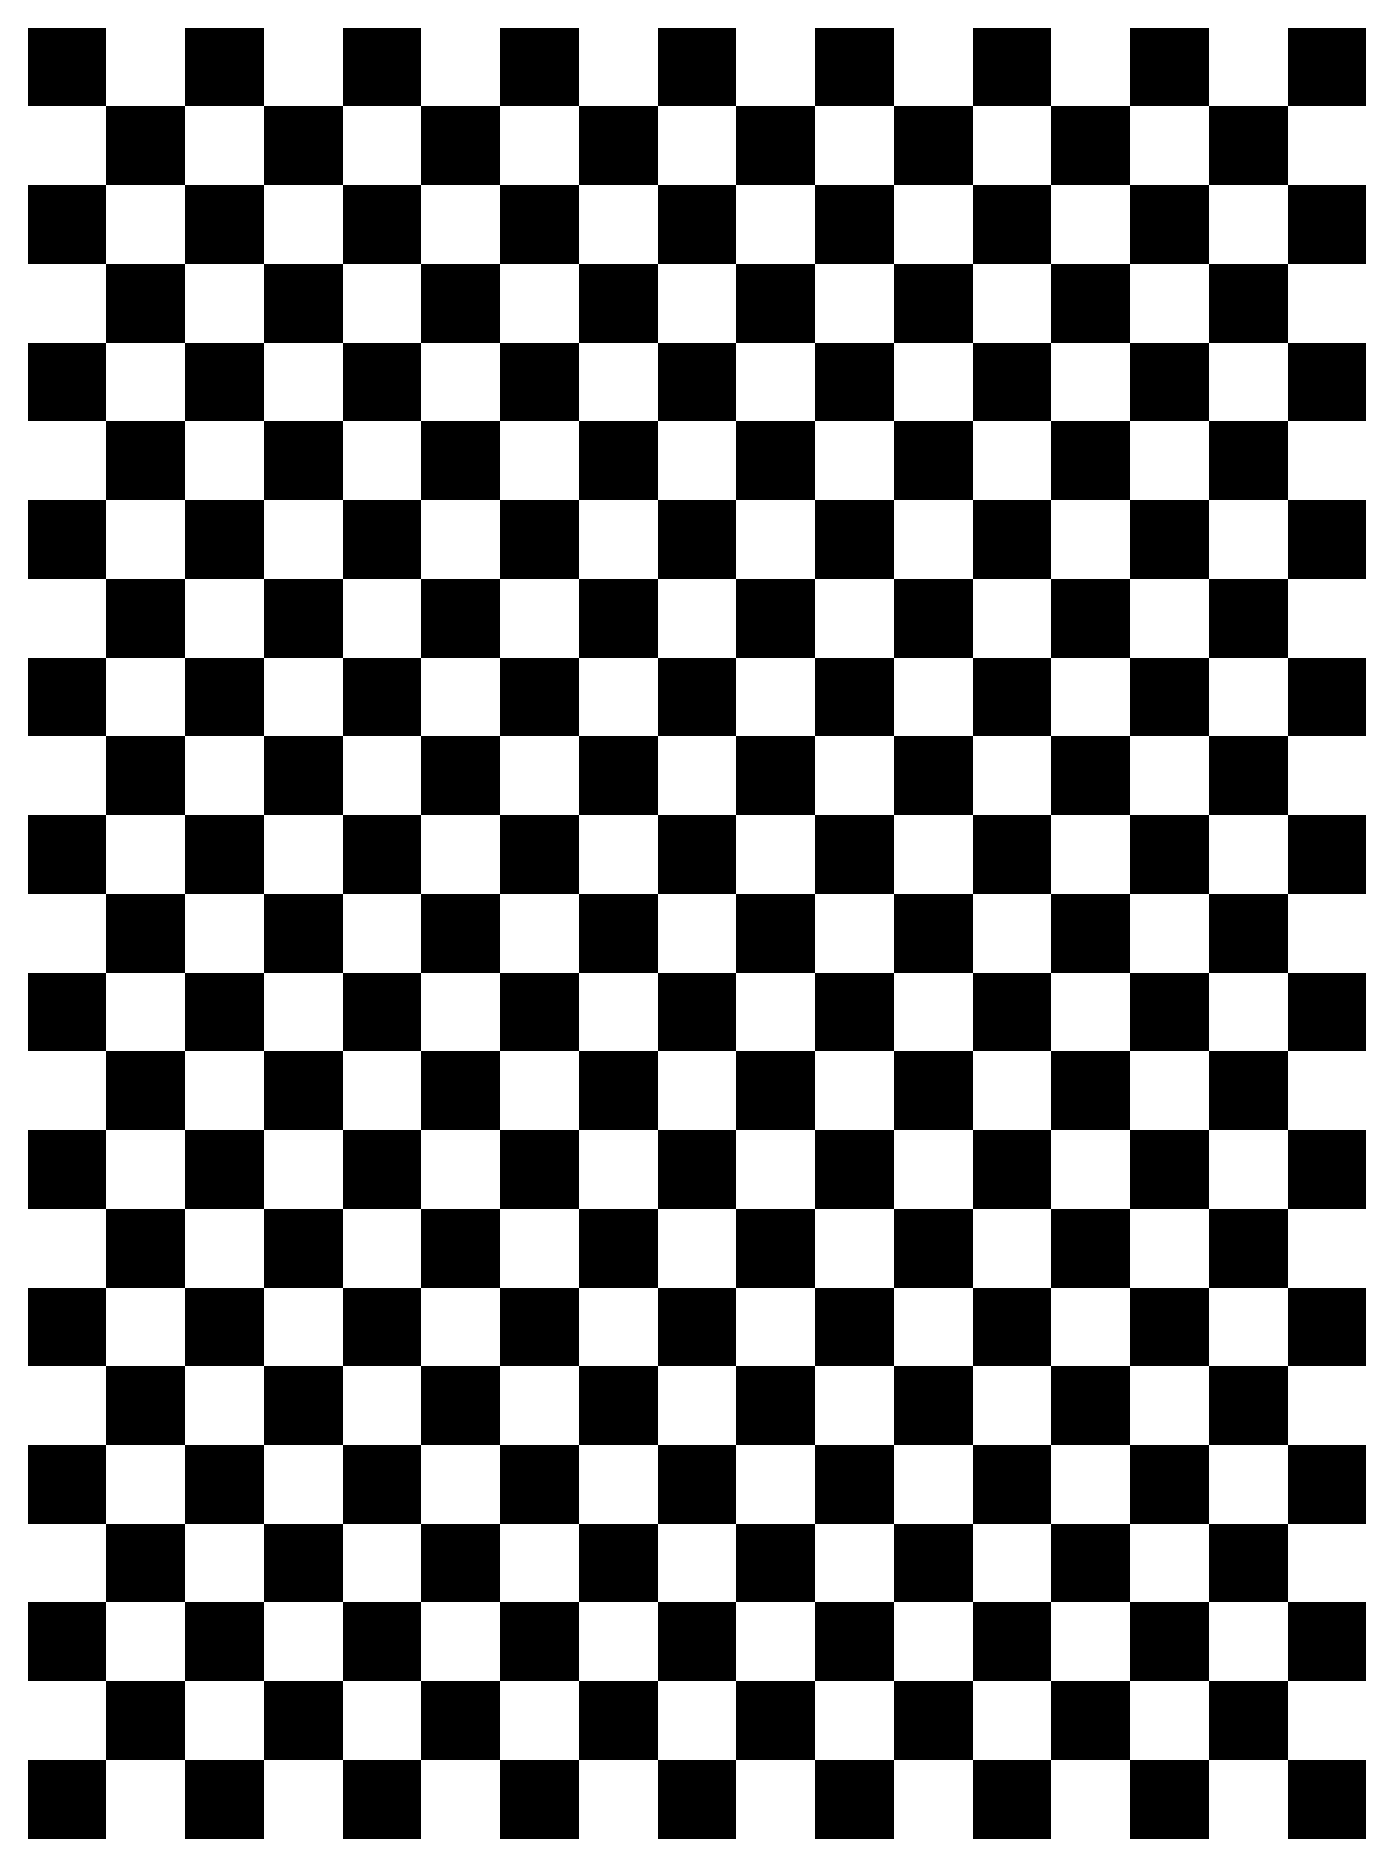
\begin{tikzpicture}[x=1cm,y=1cm]
        \foreach \x in {1,...,9}
        \foreach \y in {1,...,12}{
            \fill ({2*\x},{2*\y+1}) -- ({2*\x+1},2*\y+1) -- ({2*\x+1},2*\y) -- ({2*\x},2*\y) -- cycle ;
        }
        \foreach \x in {1,...,8}
        \foreach \y in {1,...,11}{
            \fill ({2*\x+1},{2*\y+1}) -- ({2*\x+2},{2*(\y)+1}) -- ({2*\x+2},{2*\y+2}) -- ({2*\x+1},{2*\y+2})-- cycle ;
        }
    \end{tikzpicture}
\end{center}
\vspace*{\fill}
\end{document}
